\chapter{Diseño e Implementación} % Main chapter title

\label{Chapter3} % Change X to a consecutive number; for referencing this chapter elsewhere, use \ref{ChapterX}
\definecolor{mygreen}{rgb}{0,0.6,0}
\definecolor{mygray}{rgb}{0.5,0.5,0.5}
\definecolor{mymauve}{rgb}{0.58,0,0.82}

\lstset{ %
  backgroundcolor=\color{white},   % choose the background color; you must add \usepackage{color} or \usepackage{xcolor}
  basicstyle=\large,        % the size of the fonts that are used for the code
  breakatwhitespace=false,         % sets if automatic breaks should only happen at whitespace
  breaklines=true,                 % sets automatic line breaking
  captionpos=b,                    % sets the caption-position to bottom
  commentstyle=\color{mygreen},    % comment style
  deletekeywords={...},            % if you want to delete keywords from the given language
  %escapeinside={\%*}{*)},          % if you want to add LaTeX within your code
  %extendedchars=true,              % lets you use non-ASCII characters; for 8-bits encodings only, does not work with UTF-8
  %frame=single,	                   % adds a frame around the code
  keepspaces=true,                 % keeps spaces in text, useful for keeping indentation of code (possibly needs columns=flexible)
  keywordstyle=\color{blue},       % keyword style
  language=[ANSI]C,					% the language of the code
  %otherkeywords={*,...},           % if you want to add more keywords to the set
  numbers=none,                    % where to put the line-numbers; possible values are (none, left, right)
  numbersep=5pt,                   % how far the line-numbers are from the code
  numberstyle=\tiny\color{mygray}, % the style that is used for the line-numbers
  rulecolor=\color{black},         % if not set, the frame-color may be changed on line-breaks within not-black text (e.g. comments (green here))
  showspaces=false,                % show spaces everywhere adding particular underscores; it overrides 'showstringspaces'
  showstringspaces=false,          % underline spaces within strings only
  showtabs=false,                  % show tabs within strings adding particular underscores
  stepnumber=1,                    % the step between two line-numbers. If it's 1, each line will be numbered
  stringstyle=\color{mymauve},     % string literal style
  tabsize=2,	                   % sets default tabsize to 2 spaces
  title=\lstname,                   % show the filename of files included with \lstinputlisting; also try caption instead of title
  morecomment=[s]{/*}{*/}%
}

En este capítulo se presentan la arquitectura multicore del \textit{firmware}, los mecanismos de comunicación entre procesadores y el detalle del diseño de los módulos desarrollados junto con sus interfaces.  Finalmente, se incluye una sección de trazabilidad de requerimientos con las funciones implementadas.

%----------------------------------------------------------------------------------------
%	SECTION 1
%----------------------------------------------------------------------------------------

\section{Arquitectura multicore}
\label{sec:arquitectura}

El \textit{firmware} está desarrollado sobre la base de dos proyectos vinculados del IDE MCUXpresso, uno para cada \textit{core} del microcontrolador. Para el IDE, debe haber un proyecto ``maestro'' que controle la ejecución del código (o al menos la secuencia de \textit{startup}) corriendo en el otro \textit{core}, considerado ``esclavo''.  

El proyecto maestro contiene un link al proyecto esclavo que produce que la imagen binaria del esclavo sea incluida en la imagen  binaria del maestro, cuando el proyecto maestro es compilado \citep{nxp:mcuxpresso}. De esta manera, cuando el proyecto maestro es grabado en la flash del microcontrolador, ambos proyectos son descargados a la memoria del microcontrolador.

El proyecto maestro debe ser el que se ejecuta sobre el procesador Cortex-M4 ya que el procesador Cortex-M0 permanece en estado de \textit{reset} hasta que el otro \textit{core} lo libera de este estado escribiendo un 0 en el bit M0SUB\_RST del registro RESET\_CTRL1, como se indica en el manual del microcontrolador \citep{nxp:lpc4337}.

Cuando se energiza el microcontrolador o se produce un \textit{reset}, el \textit{core} maestro inicia su secuencia de \textit{startup} y es responsable de iniciar, a su vez, la secuencia de \textit{startup} del \textit{core} esclavo.  

En las tablas \ref{tab:memoriaM4} y \ref{tab:memoriaM0} se muestra la asignación de bloques de memoria para los procesadores Cortex-M4 y Cortex-M0, respectivamente.  Puede verse que el código de cada procesador se ubica en un bloque de memoria flash independiente, los bancos A y B de 512 kB cada uno.  

Por otra parte, para evitar cualquier tipo de solapamiento en el uso de la RAM, los proyectos asociados a cada \textit{core} se linkean de forma de utilizar exclusivamente bancos de RAM separados.  En este sentido, el procesador cortex-M4 utiliza el primer bloque de RAM de 32 kB y el procesador cortex-M0 utiliza el segundo bloque de RAM de 40kB.

\begin{table}[ht]
\centering
\caption{Asignación de bloques de memoria para el Cortex-M4}
\begin{tabular}{lllll}
\toprule
\textbf{Tipo de memoria} & \textbf{Nombre} & \textbf{Alias} & \textbf{Ubicación} & \textbf{Tamaño} \\ 
\midrule
Flash                    & MFlashA512      & Flash          & 0x1a000000         & 0x80000         \\
RAM                      & RamLoc32        & RAM            & 0x10000000         & 0x8000          \\ 
\bottomrule
\end{tabular}
\label{tab:memoriaM4}
\end{table}

\begin{table}[ht]
\centering
\caption{Asignación de bloques de memoria para el Cortex-M0}
\begin{tabular}{lllll}
\toprule
\textbf{Tipo de memoria} & \textbf{Nombre} & \textbf{Alias} & \textbf{Ubicación} & \textbf{Tamaño} \\ 
\midrule
Flash                    & MFlashB512      & Flash2          & 0x1b000000         & 0x80000         \\
RAM                      & RamLoc40        & RAM2            & 0x10080000         & 0xa000          \\ 
\bottomrule
\end{tabular}
\label{tab:memoriaM0}
\end{table}

Adicionalmente, se define una zona de memoria compartida, visible por ambos procesadores para el intercambio de información. Los mecanismos de comunicación inter-procesadores (IPC, del inglés \textit{Inter Processor Communication}) se describen en la sección \ref{subsec:IPC}. 

\begin{verbatim}
/* Shared memory used by IPC */
#define SHARED_MEM_IPC   0x10088000	 
\end{verbatim}

\subsection{Inter Processor Communications}
\label{subsec:IPC}

Para comunicar ambos procesadores se utiliza una biblioteca provista por el fabricante del microcontrolador NXP, documentada en la nota de aplicación ``AN1117: Inter Processor Communications for LPC43xx'' \citep{nxp:an1117}. En este documento se explican 3 mecanismos posibles para que los dos procesadores intercambien información basados en interrupciones, en colas de mensajes y en ``casillas de correo''.  Este último método queda excluido de esta memoria por no haber sido utilizado en el desarrollo.

\subsubsection{Interrupción}
\label{subsubsec:interrupcion}

El mecanismo de interrupciones cruzadas es el más simple de los 3 métodos provistos.  Permite que un \textit{core} active una interrupción en el otro \textit{core} para enviar notificaciones cuya interpretación depende y es exclusiva de la aplicación.  El diseñador puede definir una función de \textit{callback} que es ejecutada en el contexto de la rutina de servicio de la interrupción.  

Para enviar señales al \textit{core} ``remoto'', el \textit{core} ``local'' utiliza una instrucción dedicada SEV (\textit{send event}) provista por la arquitectura Cortex.

Asimismo, dentro de la rutina de interrupción se habilita un \textit{flag} para indicar que se ha recibido una notificación IPC.  Esta variable \textit{flag} puede ser usada por las aplicaciones corriendo sobre el \textit{core} que recibe la notificación para chequear el estado de las comunicaciones. La limpieza del \textit{flag} se hace dentro de una sección crítica donde se deshabilitan temporalmente las interrupciones.  En el Cortex-M4 se enmascaran las interrupciones con mayor prioridad y en el Cortex-M0 se deshabilitan directamente, ya que este procesador no dispone del mecanismo de enmascaramiento.

El código para generar las interrupciones cruzadas utiliza dos macros. Primero \_\_DSB() (\textit{Data Syncronization Barrier}) para terminar todas las transacciones de memoria pendientes y luego \_\_SEV() (\textit{Send Event}) para generar el envío de una señal de interrupción al otro procesador.
%, como puede apreciarse en \ref{cod:interrupt}
\begin{verbatim}
/*
 * Initiate interrupt on other processor
 * Upon calling this function generates and interrupt 
 * on the other core. Ex. if called from M0 core it 
 * generates interrupt on M4 core and vice versa.
 */
static void ipc_send_signal(void)
{
  	__DSB();
  	__SEV();
}
\end{verbatim}\label{cod:interrupt}  

\subsubsection{Colas de mensajes}
\label{subsubsec:colas}

En el método de colas de mensajes, se deben definir dos áreas de memoria compartida, que se utilizan para almacenar los mensajes que cada procesador envía al otro. Una cola (búfer de comandos del \textit{host}) está dedicado a los comandos enviados del procesador maestro al esclavo, y una cola (búfer de mensajes del \textit{host}) se dedica a los mensajes que el procesador esclavo envía en respuesta al procesador maestro. La figura \ref{fig:IPC} muestra esquemáticamente esta configuración.

\vspace{10px}

\begin{figure}[ht]
	\centering
	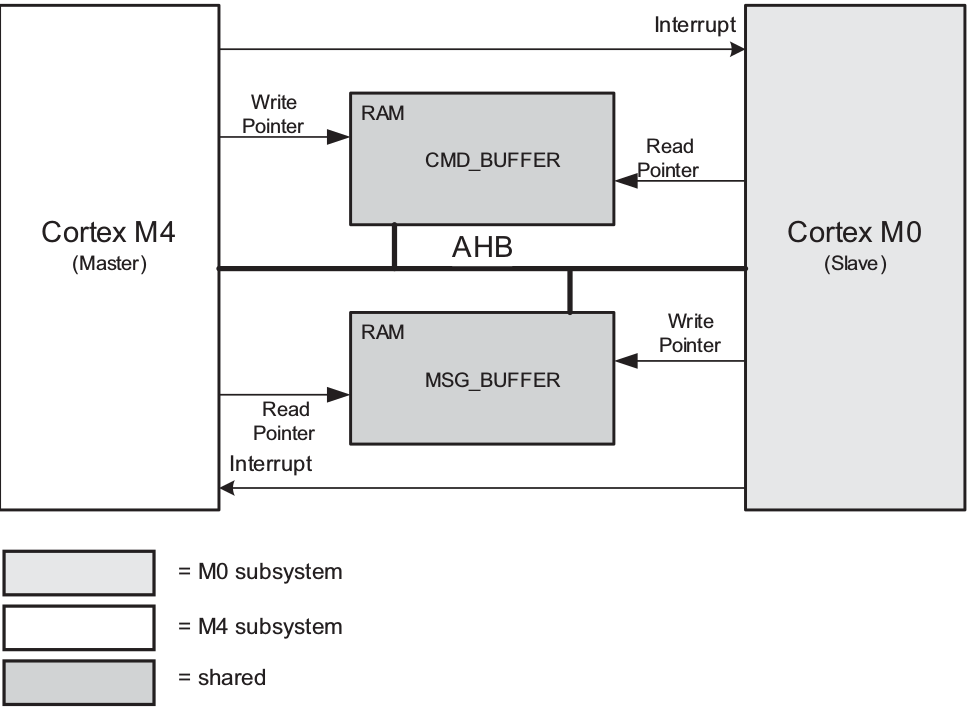
\includegraphics[width=.8\textwidth]{./Figures/IPC.png}
	\caption[Esquema de comunicación entre procesadores]{Esquema de comunicación entre procesadores basado en colas de mensajes\protect\footnotemark.}
	\label{fig:IPC}
\end{figure}

\vspace{10px}
\vfill
\footnotetext{Imagen tomada del manual de usuario del microcontrolador LPC4337 \citep{nxp:lpc4337}}

En el esquema propuesto, sólamente el procesador maestro puede escribir en el búfer de comandos y recibe los mensaje del esclavo leyendo el búfer de mensajes.  De manera análoga, únicamente el esclavo puede escribir en el búfer de mensajes y recibe comandos leyendo el búfer de comandos.

Cuando un procesador escribe un nuevo mensaje en una cola, debe notificar al otro procesador de que hay nueva información para procesar. Para tal fin, se utiliza el mecanismo de interrupción descrito en el apartado Interrupción, dentro de la subsección \ref{subsubsec:interrupcion}.  Luego de esto, el procesador que recibe el mensaje invoca a un despachador de eventos que busca en un vector de manejadores de eventos el que haya sido registrado para tal fin.

\begin{verbatim}
/* This task will receive the message from the other 
 * core and will invoke the appropriate callback with
 * the message
 */
static void ipcex_dispatch_task(void *unused)
{
  int ret;
  ipcex_msg_t msg;
  	do {
    	ret = IPC_popMsgTout(&msg, -SYS_OS_ID);
    	if((ret != QUEUE_VALID) || 
                      (msg.id.pid >= IPCEX_MAX_PID)){
      	continue;
    	}
    	if (ipcex_callback_lookup[msg.id.pid]) {
      	ipcex_callback_lookup[msg.id.pid](&msg);
    	}
  	} while (SYS_OS_ID);
}
\end{verbatim}

SYS\_OS\_ID es una macro que se utiliza para identificar el tipo de Sistema Operativo incluido en la aplicación.  En el caso particular de este trabajo, SYS\_OS\_ID es igual a 0 y esto significa que no hay Sistema Operativo.  Se debe notar que SYS\_OS\_ID = 0 implica que el despachador de eventos se ejecuta una única vez por mensaje recibido.

Para los mensajes, se define un nuevo tipo de dato ipcex\_msg\_t como una estructura que contiene información que identifica al CPU y al proceso destinararios del mensaje junto con dos campos para datos.

\begin{verbatim}
typedef struct __ipcex_msg {
  struct {
    uint16_t cpu;
    uint16_t pid;
  } id;

  uint32_t data0;
  uint32_t data1;
} ipcex_msg_t;
\end{verbatim}

\section{Diseño de módulos y definición de interfaces}
\label{sec:modulos}

El \textit{firmware} está fuertemente modularizado en archivos y utiliza un modelo de capas jerárquicas para organizar el código en distintos niveles de abstracción.  En la figura \ref{fig:capas} se pueden observar, agrupados por color, las capas utilizadas en este trabajo.  En color amarillo, el paquete de drivers provistos por el fabricante del silicio; en color naranja la capa de bibiotecas; la capa de abstracción de \textit{hardware} (HAL, por sus siglas en inglés) en color verde; y finalmente, en color celeste, la capa de aplicación con los cuatro módulos implementados.   

\begin{figure}[ht]
	\centering
	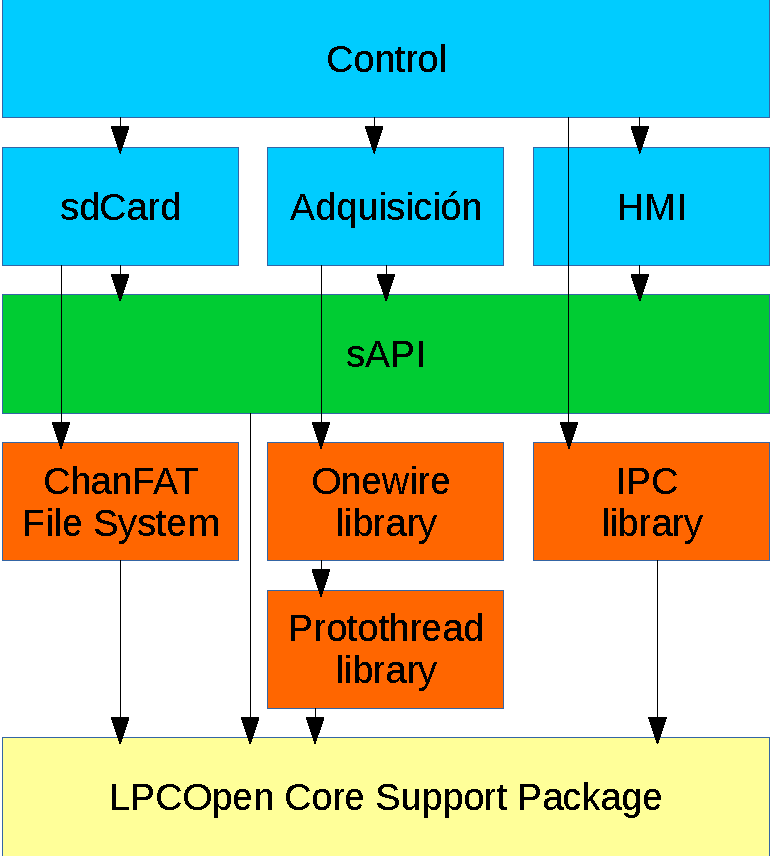
\includegraphics[width=.55\textwidth]{./Figures/capas.pdf}
	\caption[Estructura de capas para el \textit{firmware}.]{Estructura de capas para el \textit{firmware}. En orden creciente de nivel de abstracción: \textit{core support package} (amarillo), bibliotecas (naranja), sAPI (verde) y la capa de aplicación (celeste) con los 4 módulos implementados.}
	\label{fig:capas}
\end{figure}

\vspace{10px}

Para los módulos en la capa de aplicación, se confeccionó una matriz de trazabilidad de los requerimientos referidos al firmware, detallados en la sección \ref{sec:requerimientos}. La tabla \ref{tab:trazabilidad} permite saber en qué módulo del firmware serán implementados los requerimientos funcionales del proyecto.  Asimismo, permite controlar que todo este subconjunto de requerimientos sea implementado y que no haya superposición entre la funcionalidad de cada módulo.

\vspace{10px}

\begin{table}[ht]
\caption[Matriz de trazabilidad de requerimientos funcionales]{Matriz de trazabilidad de requerimientos funcionales con los módulos de \textit{firmware}}
\label{tab:trazabilidad}
\begin{tabular}{lcccc}
\toprule
\textbf{Requerimiento} & \textbf{Control} & \textbf{sdCard} & \textbf{Adquisición} & \textbf{HMI} \\ \midrule
2.1 Adquirir temperatura                   &                  &                 & X                    &              \\ %\hline
2.2 Adquirir velocidad de viento           &                  &                 & X                    &              \\ %\hline
2.3 Almacenar datos                        &                  & X               &                      &              \\ %\hline
2.4 Perfiles de consumo                    & X                &                 &                      &              \\ %\hline
2.5 Interfaz                               &                  &                 &                      & X            \\ \bottomrule
\end{tabular}
\end{table}

Se definió una estructura de control para los módulos que incluye información sobre en qué \textit{core} debe ejecutarse, un campo para identificar al módulo, un puntero a la función manejadora de eventos que es invocada cada vez que hay un mensaje para este módulo, un campo para temporizar la ejecución periódica del módulo y finalmente, un campo para el estado del módulo que puede tomar uno de los siguientes valores: DISABLE, READY o PROCESSING.

\vspace{10px}

\begin{verbatim}
typedef struct {
   CPUID_T coreID;
   moduleID_t moduleID;
   funcPtr_t eventHandler;
   tick_t period;
   moduleStatus_t status;
} module_t;
\end{verbatim}

\vspace{10px}

Toda la interacción con los módulos se realiza a través de los respectivos manejadores de eventos y una cola de mensajes como la descrita en la subsección \ref{subsubsec:colas}, pero definida en una posición de memoria no compartida, por lo que su uso se limita al \textit{core} donde está definida.

A continuación se listan los prototipos de los manejadores de eventos definidos:

\vspace{10px}

\begin{itemize}
  \item \texttt{void onewire\_handler(const ipcex\_msg\_t * msg );} 
  \item \texttt{void sdcard\_handler(const ipcex\_msg\_t * msg );} 
  \item \texttt{void hmi\_handler(const ipcex\_msg\_t * msg );} 
  \item \texttt{void control\_handler(const ipcex\_msg\_t * msg );} 
\end{itemize}

\vspace{10px}

Puede notarse que todos los manejadores reciben un mismo tipo de parámetro, un puntero constante a un mensaje de tipo \texttt{ipcex\_msg\_t}.  Cada módulo es responsable de interpretar los dos campos enteros sin signo de 32 bits de datos que contiene el mensaje.  Normalmente el campo \texttt{data0} define un comando y \texttt{data1} se utiliza opcionalmente para el envío de parámetros.

Para todos los módulos se utilizó un modelo de \textit{firmware} basado en máquinas de estados finitos (MEF) jerárquicas, donde una MEF principal controla la lógica de funcionamiento con el mayor nivel de abstracción. Los diferentes estados, a su vez, pueden o no estar modelados con MEFs dependiendo de la conveniencia de esto último.  

\section{Módulo de almacenamiento}
\label{sec:almacenamiento}

El propósito del módulo de almacenamiento es proveer al sistema de una interfaz para operar con un medio de almacenamiento no volátil que permita guardar en forma permanente los datos registrados por el módulo de adquisición y eventualmente un log con información de \textit{debug}.  

\subsection{Medio físico}
\label{subsec:mediofisico}

Se evaluaron distintas opciones de medios físicos.  En la tabla \ref{tab:medios} se recopilan las alternativas analizadas y se especifica un orden de magnitud para la capacidad de almacenamiento posible, el tipo de interfaz con el microcontrolador y el protocolo que debe implementarse en el \textit{firmware} para su utilización.

\vspace{10px}

\begin{table}[ht]
\centering
\caption{Alternativas de medios físicos evaluados.}
\label{tab:medios}
\begin{tabular}{lrcc}
\toprule
\multicolumn{1}{c}{\textbf{Medio físico}} & \multicolumn{1}{c}{\textbf{Capacidad}} & \textbf{Interfaz} & \textbf{Protocolo} \\ \midrule
USB Mass Storage Device                   & $\sim$10 Gb                            & USB 2.0           & USB                \\
Tarjeta de memoria                        & $\sim$10 Gb                            & Micro SD          & SSP                \\
Disco de estado sólido (SSD)              & $\sim$100 Gb                           & SATA III          & SATA               \\
Disco duro mecánico (HHD)                 & $\sim$1000 Gb                          & SATA III          & SATA               \\ \bottomrule
\end{tabular}
\end{table}

\vspace{10px}

Teniendo en cuenta criterios de costos y simplicidad de interacción con la CIAA-NXP, se decidió utilizar un lector de tarjetas microSD con comunicación sobre un puerto \textit{Synchronous Serial Port} (SSP).  Este protocolo es compatible con el protocolo SPI y utiliza un bus de 4 cables con las señales SCK, SSEL, MISO y MOSI.  Asimismo, el soporte seleccionado minimiza el consumo de energía comparado con las otras alternativas, lo cual lo hace deseable para la aplicación.  

El lector de tarjetas utilizado se presenta en la figura \ref{fig:lector_sdCard}, donde puede verse esquemáticamente el diagrama de conexionado entre la CIAA-NXP y el lector (figura \ref{fig:lector_conexionado}) y una vista superior del módulo de hardware (figura \ref{fig:lector_hardware}).

\vspace{20px}

\begin{figure}[h]
	\centering
	\begin{subfigure}{.5\textwidth}
		\centering
		\begin{tabular}{rll}
			\textbf{CIAA-NXP }&	& \textbf{Lector de tarjetas}\\
			+3.3V     & --\textgreater{} & +3.3V   \\
			GND       & --\textgreater{} & CS  \\
			SPI\_MOSI & --\textgreater{} & MOSI  \\
			SPI\_SCK  & --\textgreater{} & SCK \\
			SPI\_MISO & --\textgreater{} & MISO  \\
			GND       & --\textgreater{} & GND  \\
		\end{tabular}
		\caption{ }
  		\label{fig:lector_conexionado}
	\end{subfigure}%
	\begin{subfigure}{.5\textwidth}
		\centering
		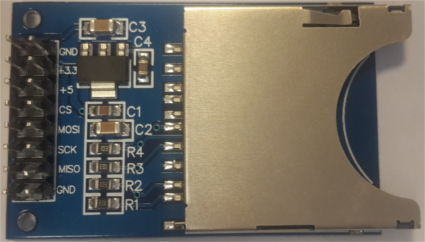
\includegraphics[width=.9\textwidth]{./Figures/sdCardReader.jpg}
		\caption{ }
		\label{fig:lector_hardware}
	\end{subfigure}
	\caption{(A) Diagrama de conexionado eléctrico y (B) Lector de tarjetas SD utilizado.}
	\label{fig:lector_sdCard}
\end{figure}

\vspace{10px}

Para la utilización del lector de tarjetas se hizo uso de la biblioteca FatFs, desarrollada por chaN \citep{fatFS}. FatFs es un módulo de sistema de archivos FAT/exFAT genérico para sistemas embebidos limitados en recursos. En la figura \ref{fig:chan} se esquematizan las interfaces de la biblioteca en una aplicación típica. 

\begin{figure}[htpb]
	\centering
	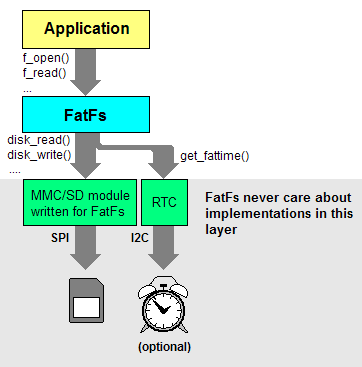
\includegraphics[width=.43\textwidth]{./Figures/chan.png}
	\caption[Diagrama de capas de fatFs]{Diagrama de capas con la ubicación de la biblioteca fatFs en el sistema y sus interfaces\protect\footnotemark.}
	\label{fig:chan}
\end{figure}

\footnotetext{Imagen tomada de \url{http://elm-chan.org/fsw/ff/doc/appnote.html}.}

El código está escrito en ANSI C y es \textit{software} libre bajo licencia estilo BSD \citep{BSD}.

\subsection{Máquina de Estados Finitos}
\label{subsec:MEFsdcard}

Se presenta el diagrama de estado de la MEF principal del módulo en la figura \ref{fig:mef_sdcard}, donde puede apreciase el punto de entrada con un circulo negro, los estado que puede tomar la máquina y las señales que provocan los cambios de estado. Se omiten del gráfico las salidas del sistema por simplicidad. 

Debe notarse que al energizarse el sistema o luego de un \textit{reset}, el módulo se encuentra deshabilitado, con la MEF en el estado \texttt{DISABLE}, del cual sólo puede salir si se recibe una señal de inicialización.  

Una vez inicializado, el módulo se encontrará la mayor parte del tiempo en el estado \texttt{IDLE} a la espera de un comando válido.  

Cuando el módulo esté realizando alguna operación de lectura, escritura o actualización sobre la tarjeta SD, el estado del módulo tendrá el valor \texttt{PROCESSING} para indicarle al módulo de control que debe tener acceso a tiempo de CPU para poder completar las operaciones pendientes.  

Todas las operación del módulo desde que es inicializado terminan incondicionalmente en el estado \texttt{IDLE}, en donde el valor de la variable que registra el estado del módulo cambia de \texttt{PROCESSING} a \texttt{READY}.

\begin{figure}[htpb]
	\centering
	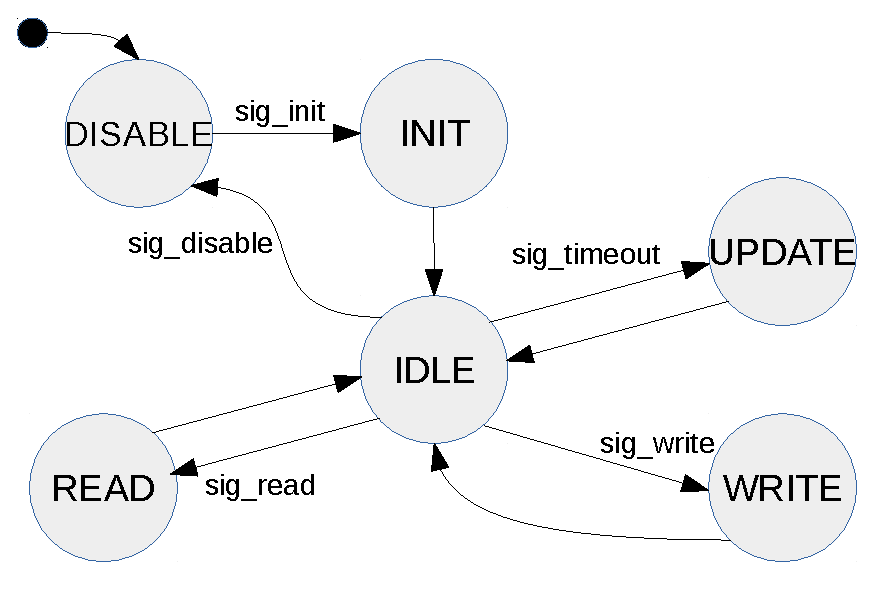
\includegraphics[width=\textwidth]{./Figures/MEF_sdCard.pdf}
	\caption[MEF principal del módulo de almacenamiento sdCard]{Máquina de estados finitos principal del módulo de almacenamiento sdCard}
	\label{fig:mef_sdcard}
\end{figure}

En la table \ref{tab:estadosAlmacenamiento} se describen cada uno de los posibles estados de la MEF principal del módulo de almacenamiento.  Asimismo, se mencionan las señales para alcanzar cada uno de los estados de la MEF y se explicitan las acciones y actividades más destacables que se realizan en cada uno de ellos.

% Please add the following required packages to your document preamble:
% \usepackage{graphicx}
\begin{table}[htpb]
\centering
\caption{Descripción de los estados de la MEF principal del módulo de almacenamiento.}
\label{tab:estadosAlmacenamiento}
\resizebox{\textwidth}{!}{%
\begin{tabular}{lll}
\toprule
\multicolumn{1}{c}{\textbf{Estado}} & \multicolumn{1}{c}{\textbf{Señal para cambio}}                                                             & \multicolumn{1}{c}{\textbf{Acciones y actividades}}                                                                                                                                                             
\\
\midrule
DISABLE                             & Reset o sig\_disable                                                                                                     & \begin{tabular}[c]{@{}l@{}}Desinicializar el controlador SPI.\\ Desinicializar la bilioteca fatFS.\\ Desinicializar el módulo de almacenamiento.\\ Cambiar el estado del módulo de READY a DISABLE.\end{tabular} \\
                                    &                                                                                                                          &                                                                                                                                                                                                                  \\
INIT                                & sig\_init                                                                                                                & \begin{tabular}[c]{@{}l@{}}Inicializar el controlador SPI.\\ Inicializar la bilioteca fatFS.\\ Inicializar el módulo de almacenamiento.\\ Cambiar el estado del módulo de DISABLE a READY.\end{tabular}          \\
                                    &                                                                                                                          &                                                                                                                                                                                                                  \\
IDLE                                & \begin{tabular}[c]{@{}l@{}} \\Transición incondicional\\ desde otros estados al \\terminar su actividad.\end{tabular} & Cambiar estado del módulo de PROCESSING a READY                                                                                                                                                                  \\
                                    &                                                                                                                          &                                                                                                                                                                                                                  \\
UPDATE                              & sig\_update                                                                                                              & Ejecutar tarea periódica de actualización de la tarjeta SD                                                                                                                                                       \\
                                    &                                                                                                                          &                                                                                                                                                                                                                  \\
WRITE                               & sig\_write                                                                                                               & \begin{tabular}[c]{@{}l@{}}\\Obtener timestamp \\ Escribir datos en la tarjeta SD\end{tabular}                                                                                                                   \\
                                    &                                                                                                                          &                                                                                                                                                                                                                  \\
READ                                & sig\_read                                                                                                                & Leer datos en la tarjeta SD                                                                                                                                                                                     \\
\bottomrule
\end{tabular}%
}
\end{table}

\clearpage
\section{Módulo de adquisición}
\label{sec:adquisicion}

El propósito del módulo de adquisición es proveer al sistema de una interfaz para operar los distintos sensores que puedan conectarse a la estación.  Originalmente, se contempló el uso de uno o varios termómetros y un anemómetro para medir temperatura del agua y velocidad del viento en superficie, respectivamente. Adicionalmente, se contempla incorporar hidrofónos para registrar el nivel de ruido submarino, principal objetivo de la estación de medición.

Se mencionó en la sección \ref{sec:objetivosyalcances}, que los hidrófonos quedaron fuera del alcance del proyecto en esta etapa del desarrollo.  De igual manera, el control del anemómetro quedará fuera de la implementación ya que se optó por priorizar el requerimiento implícito de cumplir con la fecha de entrega.  Se retoma este punto en el capítulo \ref{Chapter5}, en la sección \ref{subsec:metasnoalcanzadas}, donde se discuten sus implicancias.

Sin pérdida de generalidad, la arquitectura del módulo puede utilizarse para incorporar los sensores no implementados más adelante.

\subsection{Sensor de temperatura}
\label{subsec:1-wire}

%En la presente sección se presenta la implementación del control para el sensor de temperatura. 

Se evaluaron distintas opciones para el sensor de temperatura que estuvieran disponibles en el mercado local.  Se recopila en la tabla \ref{tab:temperatura} la información relevada para los sensores candidatos, donde puede verse fabricante y modelo de cada dispositivo junto con las principales características de interés para la aplicación.

Cabe destacar que la limitante para el rango de temperatura no es el propio sensor sino el plástico que recubre los hilos conductores que lo conectan al microcontrolador, motivo por el cual todas las alternativas evaluadas poseen rangos equivalente.  Se utiliza en la tabla un código sencillo para indicar un orden de magnitud del costo relativo del sensor con \$ para costo bajo, \$\$ para costo medio y \$\$\$ para costo alto.

% Please add the following required packages to your document preamble:
% \usepackage{graphicx}
\begin{table}[htpb]
\centering
\caption{Alternativas de sensor de temperatura evaluadas.}
\label{tab:temperatura}
\resizebox{\textwidth}{!}{%
\begin{tabular}{ccccccc}
\toprule
\textbf{Fabricante} & \textbf{Sensor} & \textbf{Tipo}                                                                    & \textbf{Precisión}      & \textbf{Rango} & \textbf{Interfaz} & \textbf{Costo} \\
\midrule
Maxim Integrated    & DS18B20         & Termómetro digital                                                               & $\pm$ 0.5 \grados C                & -55 a +125 \grados C  & 1-wire            & \$             \\
\multicolumn{1}{l}{} & \multicolumn{1}{l}{} & \multicolumn{1}{l}{}                                                             & \multicolumn{1}{l}{}    & \multicolumn{1}{l}{} & \multicolumn{1}{l}{} & \multicolumn{1}{l}{} \\
Genérico            & IM120628010     & Termistor NTC                                                                    & 1\%                     & -25 a +125 \grados C  & 1-wire            & \$             \\
\multicolumn{1}{l}{} & \multicolumn{1}{l}{} & \multicolumn{1}{l}{}                                                             & \multicolumn{1}{l}{}    & \multicolumn{1}{l}{} & \multicolumn{1}{l}{} & \multicolumn{1}{l}{} \\
TI                  & LM35            & Integrated Circuit - $\Delta V_{BE}$                                               & $\pm$ 0.5 \grados C                & -55 a +150 \grados C  & Analógica         & \$   \\
\multicolumn{1}{l}{} & \multicolumn{1}{l}{} & \multicolumn{1}{l}{}                                                             & \multicolumn{1}{l}{}    & \multicolumn{1}{l}{} & \multicolumn{1}{l}{} & \multicolumn{1}{l}{} \\
Altas Scientific    & PT-1000A        & \begin{tabular}[c]{@{}c@{}}RTD \\ (resistance temperature detector)\end{tabular} & $\pm$ (0.15 + (0.002*t)) \grados C & -55 a +125 \grados C  & Analógica         & \$\$\$         \\
\bottomrule         
\end{tabular}%
}
\end{table}

El sensor elegido es el termómetro digital DS18B20 del fabricante Maxim Integrated \citep{ds18b20}. Los motivos de la elección fueron principalmente la facilidad de uso en un entorno embebido de recursos limitados, la disponibilidad de documentación completa y detallada junto con numerosas notas de aplicación y el bajo costo del dispositivo.

En la figura \ref{fig:ds18b20_bloques} se puede apreciar un diagrama en bloques del sensor, en donde destaca la interfaz de 3 cables con una línea bidireccional de datos (DQ) y dos cables para la alimentación (GND y $V_{DD}$). 

El sensor admite una configuración de alimentación ``parásita'', en la cual se energiza desde la línea de datos DQ, lo que habilita a prescindir de un cable a costa de mayores requerimientos para la temporización de las comunicaciones y la utilización de un transistor a modo de \textit{``strong pull-up''} (conectado el bus de datos directamente a $V_{DD}$).

\begin{figure}[ht]
	\centering
	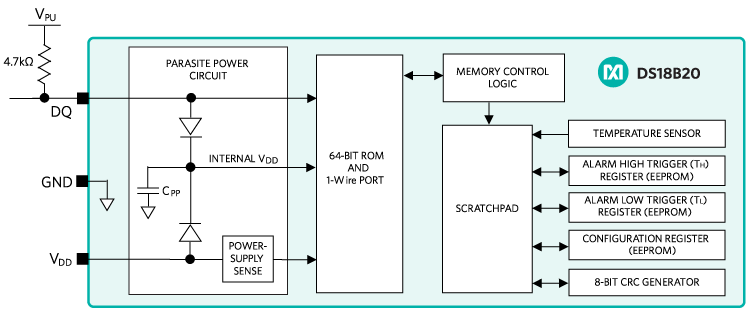
\includegraphics[width=\textwidth]{./Figures/ds18b20_bloques.png}
	\caption[Diagrama en bloques del sensor de temperatura DS18B20]{Diagrama en bloques del sensor de temperatura\protect\footnotemark.}
	\label{fig:ds18b20_bloques}
\end{figure}

\footnotetext{Imagen tomada de \url{https://www.maximintegrated.com/en/images/qv/2812.png}}

Cada sensor posee un código de identificación único de 64 bits que permite operar con múltiples sensores sobre un mismo bus de tipo 1-wire.  Mediante un algoritmo de descubrimiento se pueden identificar los sensores conectados a un mismo bus y controlarlos independientemente. 

La capacidad para identificar cuántos sensores hay conectados en cada momento y poder interrogarlos individualmente se utilizó para incorporar una funcionalidad de autochequeo, en la cual el microcontrolador es capaz de detectar si un sensor ha dejado de funcionar correctamente.

Otras características destacables son la posibilidad de configurar la resolución entre 9 y 12 bits, el uso de CRC en las comunicaciones y la capacidad para definir umbrales de alarma para los valores de temperatura medidos.

Este sensor se comercializa con distintas longitudes de cable, dentro de un encapsulado metálico sumergible.  Para este trabajo se adquirieron dos sensores sumergibles con 5 metros de cable y 2 metros de cable, respectivamente.   

Los dos sensores operan sobre una misma línea de datos con una resistencia de \textit{pull-up} de 2,2 K$\Omega$, como puede verse en el diagrama de conexionado eléctrico de la figura \ref{fig:ds18b20_conexionado}.  El encapsulado sumergible puede apreciarse en la figura \ref{fig:termometro}.

\vspace{10px}

\begin{figure}[ht]
	\centering
	\begin{subfigure}{.6\textwidth}
		\centering
		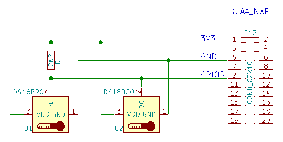
\includegraphics[height=4cm]{./Figures/ds18b20_conexionado.pdf}
		\caption{ }
  		\label{fig:ds18b20_conexionado}
	\end{subfigure}%
	\begin{subfigure}{.4\textwidth}
		\centering
		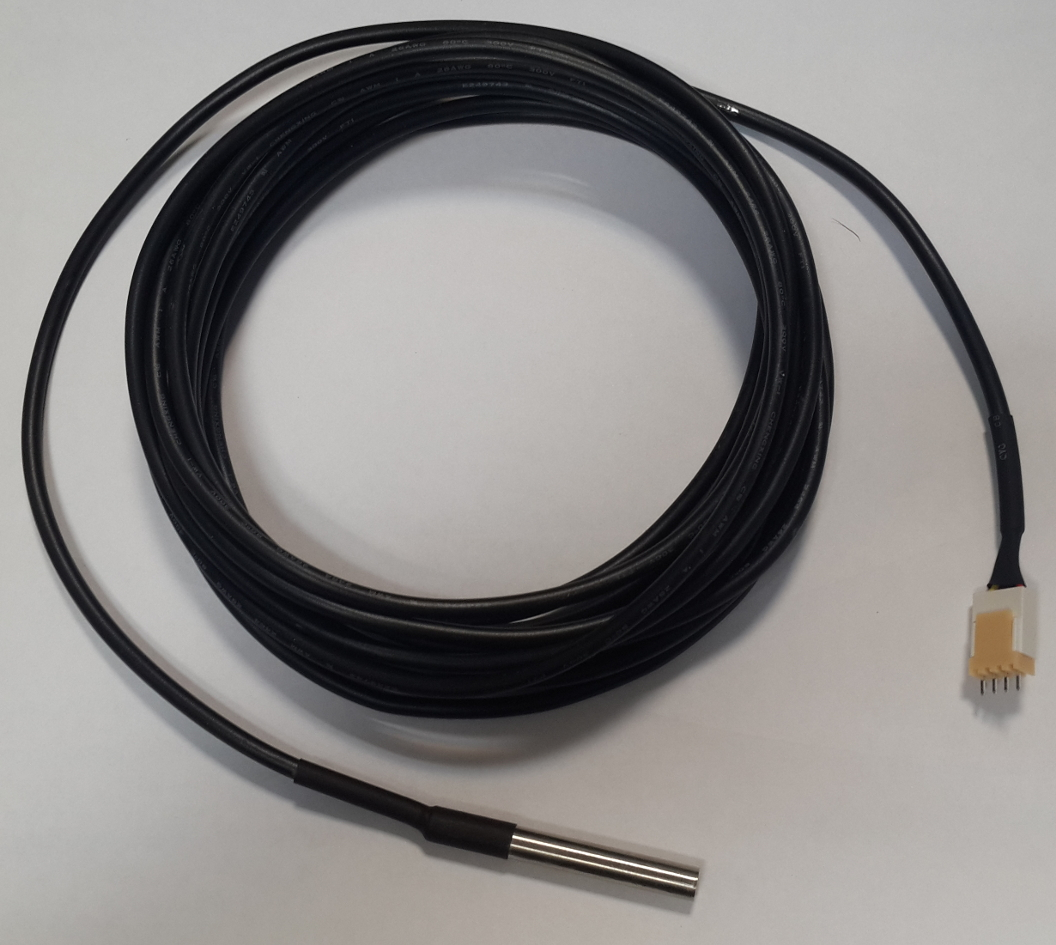
\includegraphics[height=4cm]{./Figures/ds18b20.jpg}
		\caption{ }
		\label{fig:termometro}
	\end{subfigure}
	\caption{(A) Diagrama de conexionado eléctrico y (B) Sensor de temperatura utilizado.}
	\label{fig:ds18b20}
\end{figure}

Para el control de los dispositivos se adaptó una implementación de controlador de bus \textit{1-wire} para microcontroladores de la familia LPC1343, desarrollada en forma de biblioteca por James Harwood \citep{harwood}.  En esta biblioteca se hace uso de las técnicas de programación concurrente descritas en el capitulo \ref{Chapter2}, subsección \ref{subsec:protothreads}.

\subsection{Máquina de Estados Finitos}

En forma análoga a lo presentado en la subsección \ref{subsec:MEFsdcard}, se muestra aquí el diagrama de estado de la MEF principal del módulo en la figura \ref{fig:mef_adquisicion}, donde puede apreciase el punto de entrada con un circulo negro, los estado que puede tomar la máquina y las señales que provocan los cambios de estado. Se omiten del gráfico las salidas del sistema por simplicidad. 

Igualmente, debe notarse que al energizarse el sistema o luego de un \textit{reset}, el módulo se encuentra deshabilitado, con la MEF en el estado \texttt{DISABLE}, del cual sólo puede salir si se recibe una señal de inicialización.  

Una vez inicializado, el módulo se encontrará la mayor parte del tiempo en el estado \texttt{IDLE} a la espera de un comando válido.  

Cuando el módulo esté realizando alguna operación de adquisición, configuración o autochequeo sobre los sensores conectados, el estado del módulo tendrá el valor \texttt{PROCESSING} para indicarle al módulo de control que debe tener acceso a tiempo de CPU para poder completar las operaciones pendientes.  

Todas las operación del módulo desde que es inicializado terminan incondicionalmente en el estado \texttt{IDLE}, en donde el valor de la variable que registra el estado cambia de \texttt{PROCESSING} a \texttt{READY}.

\begin{figure}[htpb]
	\centering
	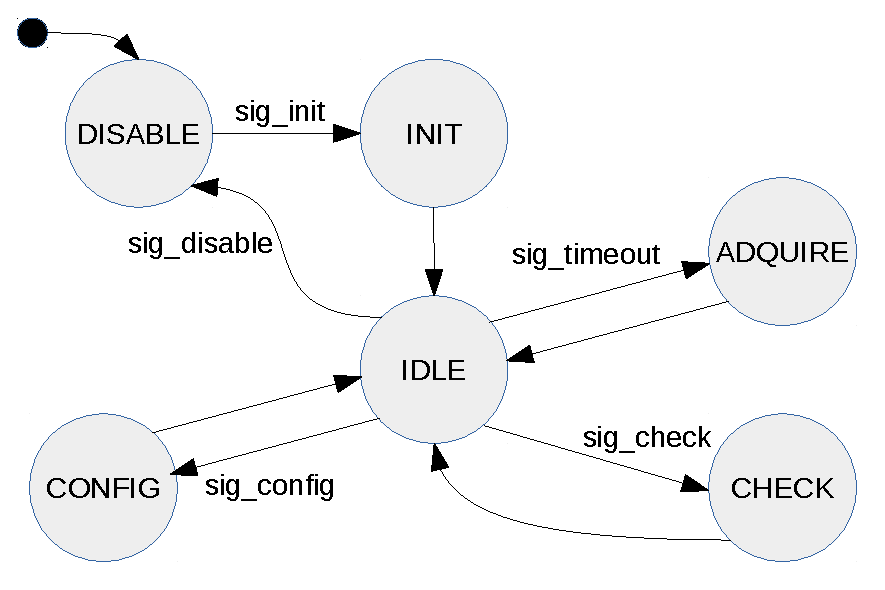
\includegraphics[width=\textwidth]{./Figures/MEF_adquisicion.pdf}
	\caption[MEF principal del módulo de adquisición de temperatura]{Máquina de estados finitos principal del módulo de adquisición de temperatura}
	\label{fig:mef_adquisicion}
\end{figure}
%\subsection{Sensor de velocidad de viento}
%\label{subsec:anemometro}

\section{Módulo interfaz HMI}
\label{sec:HMI}

\section{Módulo de control}
\label{control}
